\documentclass[10pt,final,a4paper,oneside,onecolumn]{article}

%%==========================================================================
%% Packages
%%==========================================================================
\usepackage[a4paper,left=3.5cm,right=3.5cm,top=3cm,bottom=3cm]{geometry} %% change page layout; remove for IEEE paper format
\usepackage[T1]{fontenc}                        %% output font encoding for international characters (e.g., accented)
\usepackage[cmex10]{amsmath}                    %% math typesetting; consider using the [cmex10] option
\usepackage{amssymb}                            %% special (symbol) fonts for math typesetting
\usepackage{amsthm}                             %% theorem styles
\usepackage{dsfont}                             %% double stroke roman fonts: the real numbers R: $\mathds{R}$
\usepackage{mathrsfs}                           %% formal script fonts: the Laplace transform L: $\mathscr{L}$
\usepackage[pdftex]{graphicx}                   %% graphics control; use dvips for TeXify; use pdftex for PDFTeXify
\usepackage{array}                              %% array functionality (array, tabular)
\usepackage{upgreek}                            %% upright Greek letters; add the prefix 'up', e.g. \upphi
\usepackage{stfloats}                           %% improved handling of floats
\usepackage{multirow}                           %% cells spanning multiple rows in tables
%\usepackage{subfigure}                         %% subfigures and corresponding captions (for use with IEEEconf.cls)
\usepackage{subfig}                             %% subfigures (IEEEtran.cls: set caption=false)
\usepackage{fancyhdr}                           %% page headers and footers
\usepackage[official,left]{eurosym}             %% the euro symbol; command: \euro
\usepackage{appendix}                           %% appendix layout
\usepackage{xspace}                             %% add space after macro depending on context
\usepackage{verbatim}                           %% provides the comment environment
\usepackage[dutch,USenglish]{babel}             %% language support
\usepackage{wrapfig}                            %% wrapping text around figures
\usepackage{longtable}                          %% tables spanning multiple pages
\usepackage{pgfplots}                           %% support for TikZ figures (Matlab/Python)
\pgfplotsset{compat=1.14}						%% Run in backwards compatibility mode
\usepackage[breaklinks=true,hidelinks,          %% implement hyperlinks (dvips yields minor problems with breaklinks;
bookmarksnumbered=true]{hyperref}   %% IEEEtran: set bookmarks=false)
%\usepackage[hyphenbreaks]{breakurl}            %% allow line breaks in URLs (don't use with PDFTeX)
\usepackage[final]{pdfpages}                    %% Include other pdfs
\usepackage[capitalize]{cleveref}				%% Referensing to figures, equations, etc.
\usepackage{siunitx}								%% Appropriate behavior of units
\usepackage[utf8]{inputenc}   				 	%% utf8 support (required for biblatex)
\usepackage{csquotes}							%% Quoted texts are typeset according to rules of main language
\usepackage[style=ieee,doi=false,isbn=false,url=false,date=year,mincitenames=1,maxcitenames=2,minbibnames=15,maxbibnames=15,backend=biber]{biblatex}
%\renewcommand*{\bibfont}{\footnotesize}		%% Use this for papers
\setlength{\biblabelsep}{\labelsep}
\bibliography{../../bib}

%%==========================================================================
%% Define reference stuff
%%==========================================================================
\crefname{figure}{Figure}{Figures}
\crefname{equation}{}{}

%%==========================================================================
%% Define header/title stuff
%%==========================================================================
\newcommand{\progressreportnumber}{32}
\renewcommand{\author}{Erwin de Gelder}
\renewcommand{\date}{July 2, 2020}
\renewcommand{\title}{Performance assessment of automated vehicles using real-world driving scenarios}

%%==========================================================================
%% Fancy headers and footers
%%==========================================================================
\pagestyle{fancy}                                       %% set page style
\fancyhf{}                                              %% clear all header & footer fields
\fancyhead[L]{Progress report \progressreportnumber}    %% define headers (LE: left field/even pages, etc.)
\fancyhead[R]{\author, \date}                           %% similar
\fancyfoot[C]{\thepage}                                 %% define footer



% Table stuff
\usepackage{booktabs}
\newcommand{\otoprule}{\midrule[\heavyrulewidth]}

\begin{document}
	
\begin{center}
	\begin{tabular}{c}
		\title \\ \\
		\textbf{\huge Progress report \progressreportnumber} \\ \\
		\author \\ 
		\date
	\end{tabular}
\end{center}

\section{Previous meeting minutes}

\begin{itemize}
	\item We discussed the PowerPoint version of the work done for the scenario risk quantification.
\end{itemize}

\section{Summary of work}

\begin{itemize}
	\item I checked the progress on the Doctoral Education Programme. I have completed the required 15 graduate school credits for the research skills and the discipline-related skills. For the transferable skills, I still need 2.5 Graduate School (GS) credits. I plan to follow the following courses:
	\begin{itemize}
		\item T1.C3 (1 GS credit): Sharing your Research and work as Simple as a TEDxTalk
		\item T4.G11 (0.5 GS credits): LinkedIn for PhDs
		\item T4.G5 (1 GS credit): Career Development -- Personal Branding, Presenting Yourself Effectively
	\end{itemize}
	Note that it is mandatory to have 1 GS credit for a ``career development'' course.
	
	\item Ontology for scenarios for the assessment of automated vehicles:
	\begin{itemize}
		\item I received a response from Larry Head, the editor of Transportation Research Part C. He does not want to reconsider the decision, because the editor also thinks the paper is not ``significant enough to be accepted''.
		
		\item I spoke with Steven Kraines, an expert researcher in ontologies and, more specifically, the Web Ontology Language (OWL). He liked the article, but he had also some good comments. His main comment is that because we use Unified Modeling Language (UML) instead of OWL, it is more used to ``model the world'' whereas OWL is more about ``understanding the world''. In his opinion, the strength of an ontology is that it can be used by an agent (i.e., a computer) to understand the world, e.g., to classify objects and to identify relationships between objects. However, because we used UML, he sees it more as an effort to unambiguously describe [synthesized] scenarios. 
		
		\item I agree with the view of Steven Kraines. He offered his help to describe the ontology in OWL. Also, he made some other suggestions to redefine few terms. He offered to help revising the paper accordingly. I am positive on exploring this further with him. 
		
		\item However, since work like this (or perhaps this is true all research work) is never fully finished, I do not want to put (again) a lot of effort in it before submitting a paper. Therefore, I propose to submit the current paper with only slight adaptations and to have a potential new paper as a follow up. I propose the following adaptations:
		\begin{itemize}
			\item Although technically speaking, we are still presenting an ontology, I propose to remove the word ontology from the paper as we do not make full use of the potentials of ontologies. Instead, our ontology is used to come to an object-oriented representation of a scenario and its attributes. As a title, I propose ``Object-oriented view on scenarios for the assessment of automated vehicles''\footnote{The original title is ``Ontology for scenarios for the assessment of automated vehicles''.}, as this is closer to the actual contribution of the paper.
			
			\item Even the section ``why an ontology'' can remain if we substitute ``ontology'' by ``object-oriented'' and do some rephrasing to make it grammatically correct. In this way, we directly address the first and third comment of the reviewer.
			
			\item To address the fourth comment of the reviewer (``Since the presented theory hasn't been really implemented and tested, it is not really obvious how usable the presented theory is in practice''), I do not see an easy way to address that within the paper other than simply stating that the theory has been implemented and tested. However, what I can do, is to add more examples on our code at GitHub. Furthermore, I would like to add a Jupyter Notebook\footnote{A Jupyter Notebook is a document that contains live code, equations, visualizations, and text.} in which I clearly explain all features of the implementation and to demonstrate how this can be usable in practice\footnote{As a benefit, this will also serve as a good introduction for other TNO users of the code.}.
			
			\item I still have to find a suitable journal. The previous editor suggested to resubmit or to submit the paper to Transportation Research Part A: Policy and Practice. I assumed resubmitting is out of the question. And the latter option does not seem suitable as I cannot easily find papers of Transportation Research Part A that are relevant to our work.
		\end{itemize}
	\end{itemize}

	\item Scenario risk quantification:
	\begin{itemize}
		\item I made quite some progress on the case study for the work on the scenario risk quantification. 
		
		\item In the first case study, I consider the scenario where a vehicle in front of the ego vehicle is braking. Three parameters are considered: the starting speed, the speed difference, and the average deceleration. Based on the original data set \autocite{paardekooper2019dataset6000km}, the joint probability density function is estimated. Since visualization is easier with only two free parameters, I fixed the starting speed at \SI{20}{\meter\per\second}. \Cref{fig:original pdf} shows the conditional joint probability density function with the given aforementioned starting speed. In case of a human driver\footnote{The human driver is modeled using a combination of the Human Driver Meta-Model \autocite{treiber2006delays} and the Intelligent Driver Model plus \autocite{schakel2010effects}.}, from a Monte Carlo simulations with 1000 parameter evaluations, it appeared that there is a probability of a collision of $4.7 \cdot 10^{-3} \pm 1.9 \cdot 10^{-3}$.
		
		\begin{figure}
			\centering
			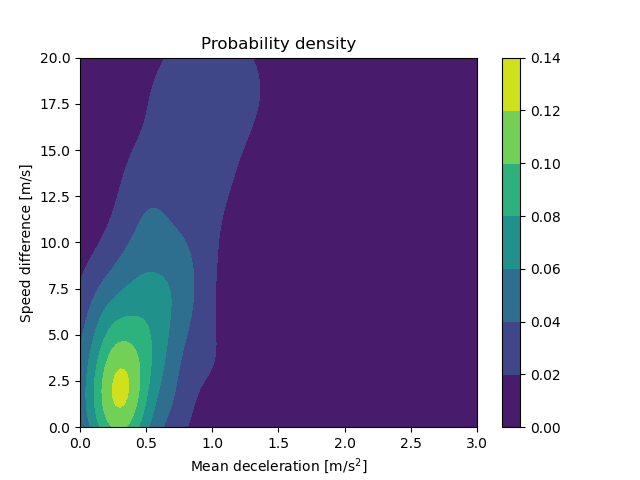
\includegraphics[width=.8\linewidth]{orig_pdf}
			\caption{The joint probability density of the two parameters considered in the first case study.}
			\label{fig:original pdf}
		\end{figure}
	
		Based on some work of a student at TNO that I am supervising, it is possible to determine relatively efficiently an importance density from which we can sample instead of the original density. The idea of the student is based on the Marching Cubes algorithm \autocite{lorensen1987marching} extended to higher dimensions \autocite{bhaniramka2004isosurface}. For this example, the importance density is shown in \cref{fig:importance pdf}. When doing simulations with only 50 parameter evaluations, the estimated probability of a collision if $5.5 \cdot 10^{-3} \pm 3.1\cdot 10^{-4}$. This demonstrates that the importance sampling greatly reduces the number of simulations. \Cref{tab:results} summarizes the result of the importance sampling.
		
		\begin{figure}
			\centering
			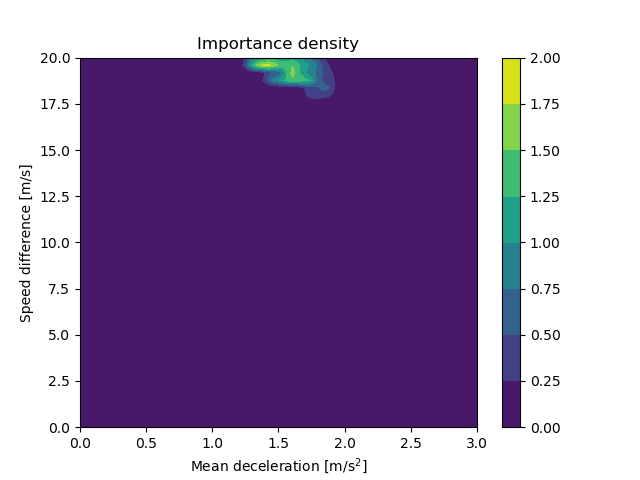
\includegraphics[width=.8\linewidth]{is_pdf}
			\caption{The importance density of the two parameters considered in the first case study.}
			\label{fig:importance pdf}
		\end{figure}
	
		\begin{table}
			\centering
			\caption{Results of the case study with two parameters.}
			\label{tab:results}
			\begin{tabular}{llll}
				\toprule
				Sampling density & Number of samples & Mean result & Standard deviation \\ \otoprule
				Original density (\cref{fig:original pdf}) & 1000 & 0.0047 & 0.0019 \\
				Importance density & 50 & 0.0055 & 0.0003 \\
				\bottomrule
			\end{tabular}
		\end{table}
	
		\item The example above is executed with a model of a driver. Next, I want to redo the experiment with (a simplified model of) an automated driving system (ADS), such as an adaptive cruise control (ACC). In \autocite{kesting2010enhanced}, an ideal ACC is presented, so my idea is to use that one.
		
		\item Next, I want to combine the driver with the ADS. As far as I know, there is not much literature about how to model the combination of a human driver and an ADS. In a rather recent publication, \textcite{varotto2018modelling} model what a driver will do when driving with an ACC: either continue without intervention, increase the set speed, decrease the set speed, use the throttle, or disengage the system. It is a rather complex model (many equations involved), but because this was the only publication I could find, I would like to implement it next to driver model and the ACC model. 
		
		\item Instead of only looking at the probability of a collision, I also want to consider the potential harm in case there is a collision. I found few articles in which a regression model is obtained for estimating the probability of a serious injury based on the impact speed \autocite{augenstein2003methodology, yoshida2016development}. I think these regression models can be directly applied in the case study.
	\end{itemize}

	\item Test case generation: In the previous meeting, I mentioned that I had some new ideas to improve the method of generating test cases. I implemented these methods and for the rather simplistic case study, it seems to work. I still have some questions if I want to make the method more generally applicable. Nevertheless, I am very happy with the results so far. Due to lack of time, I will not further elaborate on the method. During the next progress meeting, we can discuss this in more detail.
\end{itemize}

\section{Future plans}

In \cref{fig:planning}, the planning is shown. There are no changes compared to the planning shown in the previous report. During the next progress meetings, I want to update the planning and discuss this in more detail.

For now, I plan to do the following:
\begin{itemize}
	\item Revise the ``ontology'' paper and providing a better documentation of the code on GitHub.
	\item For the scenario risk quantification:
	\begin{itemize}
		\item Implement the model of the interaction between the driver and the ACC.
		\item Perform the case study for cut-in scenarios.
		\item Start writing the method section of the article.
	\end{itemize}
	\item Describe the method for generating the test cases.
\end{itemize}

\begin{figure}
	\centering
	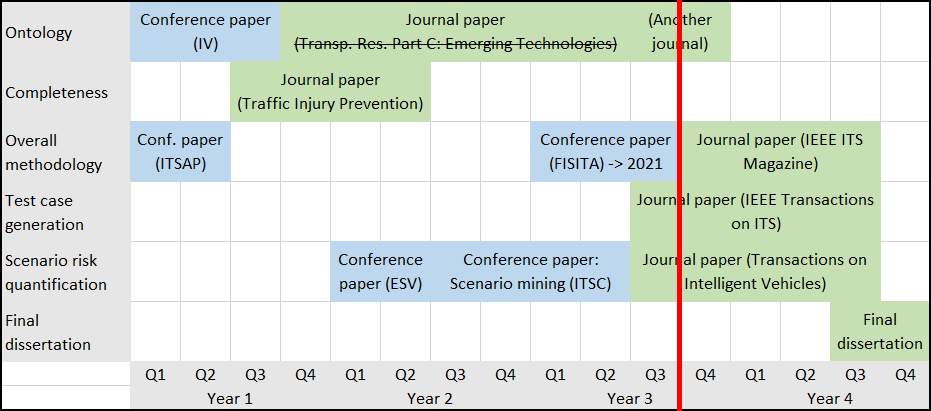
\includegraphics[width=\linewidth]{planning.png}
	\caption{Proposed planning at the time of this report. The red line indicated the time when writing this report.}
	\label{fig:planning}
\end{figure}


\printbibliography

%\clearpage
%\includepdf[pages=-,pagecommand={},width=\paperwidth]{../../""/.pdf}

\end{document}